%======================================================================
\chapter{Introduction}\label{ch1:Intro}

\markright{Introduction}
%======================================================================

\paragraph{Curiosity/phenomenology} Paragraph that will tell the reader that hydrogels are cool.

\paragraph{Applications/Market size of the applications sectors} If the previous paragraph does not convince the reader, well my last hope is that money does.

Besides, because of such a wide variety of response triggers, hydrogels can serve as sensors or actuators or can be utilized in controlled drug delivery systems, biosensors, tissue engineering scaffolds, and others [20], because of their biomimetic properties and multi functionalities [21]\citep{bustamantetorresHydrogelsClassificationAccording2021}.

In particular, biomedical applications are very popular and include cell culture [5], wound dressing and healing [2,6], drug delivery [2,7,8], tissue engineering scaffolds [9], bone repair [10], and cartilage regeneration [11]\citep{picchioniHydrogelsBasedDynamic2018}. 
 

\paragraph{Description of the Thesis} What the reader will find in each chapter and section.

\paragraph{Why computers and not rheometers?} Explain how in silico experiments can help to understand the relation between the network and the mechanical response.

\section{State of the art: Hydrogels}\label{ch1:StateArt}

\begin{itemize}
    \item Characteristics
    \item Descriptions 
    \item Synthesis techniques
    \item Cross-linking (Bond breaking)
\end{itemize}

\paragraph{General description of a hydrogel}
A hydrogel is commonly describe as a material composed by a network of polymers chains that exhibits the abilitiy to swell and retain a significant fraction of water within its structure, but will not dissolve in water\citep{ahmedHydrogelPreparationCharacterization2015a,ahmedHydrogelsMicrogelsDriving2025,priyaComprehensiveReviewHydrogel2024,bustamantetorresHydrogelsClassificationAccording2021}.\footnote{the main difference with the microgels, is the size. Hydrogel is bulk, and microgelgel is particle.}
The water absorption capacity, network stability of hydrogels, and the conformation of the network with polymer chains are attributable to crosslinking mechanisms\citep{priyaComprehensiveReviewHydrogel2024,ahmedHydrogelPreparationCharacterization2015a}.
Meanwhile, the polymer chains are predominantly composed with hydrophilic functional groups and can be modified to suit a variety of applications\citep{ahmedHydrogelPreparationCharacterization2015a,priyaComprehensiveReviewHydrogel2024,bustamantetorresHydrogelsClassificationAccording2021}.

% Hydrophilic polymers might be considered as those polymers that contain polar functional groups such as hydroxyl (-OH), carboxyl (-COOH), and amino (-NH2) groups that make them soluble or swelled by water.

While the analysis of the impact of functional groups is important, the present project prioritizes the examination of mechanisms that are more pertinent to the mechanical response. 
The crosslinking mechanisms\footnote{The hydrogels are prepared using different methods like chemical cross-linking of monomers, physical cross-linking using temperature or pH changes, and blending of natural or synthetic polymers.}, in particular, are of particular interest, as they are responsible for resisting dissolution. 
This suggests that crosslinking mechanisms enable the network to undergo modification by external stimuli.

The subsequent sections will present the essential information to facilitate a comprehensive understanding of the crosslinking mechanisms, their relationship to the mechanical response, the reported mechanical response of hydrogels, and the correlation between rheology experiments and stress curves.


\section{Polymeric Structure}

\paragraph{Overview} The chemical and topological structure of polymer networks are interconnected, influencing their overall characteristics.
The chemical structure is defined by the chemical composition of the network components. 
Tuning this structure effectively enables the incorporation of functions to polymer networks.
In contrast, polymer network topology refers to the configuration of junctions and strands within a polymer network.
Given that many properties of polymer networks (e.g., elasticity, porosity, and swellability) have topological origins, there is growing interest in understanding and controlling polymer network topology from a molecular perspective\citep{guPolymerNetworksPlastics2020}.

\paragraph{Length scales} Those properties can be explained in terms of topological features across different length scales, ranging from the molecular to the submicron scale.
From 10–100 nm, polymer network topology is characterized by inhomogeneity in junction/strand density (Figure~\ref{fig:lengthScales}), which results from concentration fluctuations during network formation\footnote{Small-angle scattering techniques provide semi-quantitative information at this length scale (see below).[21,22]} [20].
From 1–10 nm, dangling/unreacted strands and/or junctions, entanglements, and loops of various orders\footnote{Dangling chains, occur when a reactive group from the network precursors remains unreacted after network formation, meanwhile, the loops are cyclic structures defined by the number of strands and junctions in the cycle. 
} comprise the macromolecular features that dominate network structure\footnote{Although they contain rich topological information, conventional scattering and spectroscopic methods fail to characterize these macromolecular features.[23]} (Figure~\ref{fig:lengthScales}). 
From less than a nanometer, network features are primarily dictated by chemistry rather than topology; branch functionality, however, is a critical molecular-scale feature that dictates network topology (Figure~\ref{fig:lengthScales}). 
While branch functionality is difficult to characterize experimentally\footnote{To characterize the topological features in amorphous regions of polymer networks, theory/ simulation, swelling experiments, and mechanical tests are often used.}, it can typically be predicted based on the functionality of network precursors\citep{guPolymerNetworksPlastics2020}.

\begin{figure}[ht!]
    \centering
    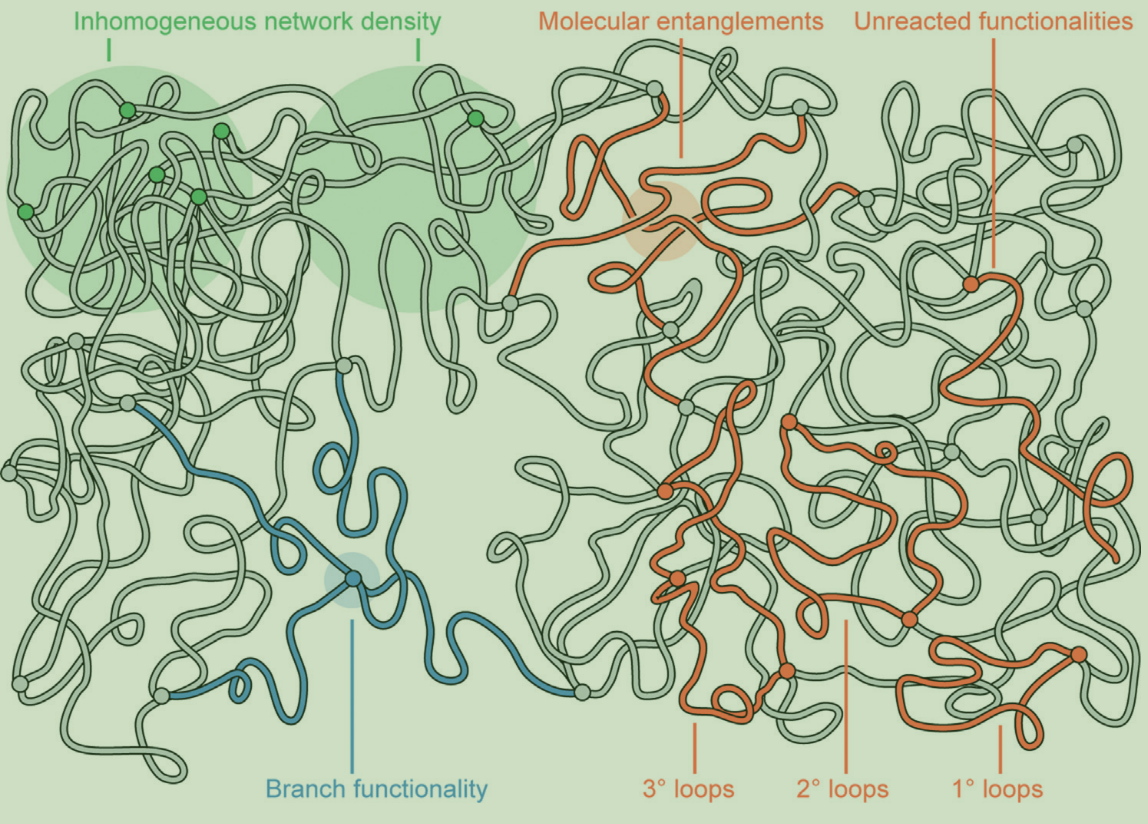
\includegraphics[width=0.8\textwidth]{figs/multilengthTopology.png}
    \caption{Multilength stuff. Scale from 10 to 100 nm shown in green, 1 to 10 nm shown in red and <1 nm shown in blue. }\label{fig:lengthScales}
\end{figure}

\subsection{Basic properties of Polymer Networks} 

\paragraph{Elasticity} The physical explanation of rubber elasticity comes from the reduction in conformational entropy that occurs as a strand in a network is stretched, this process is often modeled as the unwinding of flexible, random coils. 
Once the external stretching force is removed, an elastic entropic force restores the strands to their unstretched and higher entropy state. 
Therefore, it is concluded that network strands act as entropic molecular springs\citep{guPolymerNetworksPlastics2020}. 

\paragraph{Swelling} Polymer networks constructed from strong (e.g., covalent) bonds typically do not dissolve in solvents. 
Instead, such networks absorb solvent up to an equilibrium concentration and undergo a concomitant increase in volume. 
The equilibrium degree of swelling is dictated by a balance between the free energy of polymer-solvent mixing and the free energy cost of expanding the network, which is expressed by the Flory–Rehner equation[11,133]\footnote{for isotropic swelling of an affine polymer network [Eq. (12)]:
    \begin{gather*}
        \ln(1-\phi_{\mathrm{eq}}) + \phi_{\mathrm{eq}} + \xi\phi^2_{eq} = \eta_{eff}V_1(\phi_{\mathrm{eq}}/2-\phi^{1/3}_{eq})
    \end{gather*}
}

\paragraph{Viscoelasticity} Polymeric materials exhibit both viscous and elastic characteristics upon deformation, meaning that their properties may vary with the time scale or frequency at which measurements are performed. 
To characterize this viscoelasticity with respect to tensile, compressive, or shear deformation, several types of experimental measurements are commonly applied, such as stress relaxation, creep, and oscillatory shear tests\citep{guPolymerNetworksPlastics2020}. 

\subsection{Structure and mechanical response}




\paragraph{Covalent Adaptable Networks} Covalent adaptable networks (CANs) are produce by incroporating dynamic covalent bonds into convalent polymer networks, which alows for stimulus-induced reconfiguration of networks to reduce stresses or heal damage.
As a result, CANs not only exhibit the robust mechanical properties typical of thermosets but they can also possess the processability and relaxation behavior of thermoplastics.
Depending on the exchange mechanism, CANs may be further classified into two groups: dissociative CANs and associative CANs\citep{guPolymerNetworksPlastics2020}\footnote{A distinguishing characteristic between dissociative and associative CANs is that associative CANs display a constant crosslinking density with respect to temperature.
Since the rate of stress relaxation of these networks depends on the rate of bond rearrangement, the associative bond exchange mechanism is reflected in a viscosity with Arrhenius-like temperature dependence (Figure 9 C).
}.

\paragraph{Microporus Polymer Networks} Microporous materials are defined as materials containing interconnected pores of less than 2 nm in diameter on average. 
Due to their large surface area, many conventional microporous materials (e.g., zeolites, activated carbons) are widely used as catalysts, sorbents, and separation membranes. 





\begin{comment}
Due to their strong bonds, covalent polymer networks possess high mechanical strength across a wide range of conditions. 

While such mechanical stability enables their use in daily life, 

Many emerging applications and environmental sustainability concerns demand unconventional properties of polymernetworks, such as reprocessability, repairability upon damage, and adaptability to different environments.


Polymer networks with rapid stress relaxation that can heal when damaged (“self-healing”) are often constructed from non-covalent network bonds (e.g., metal–ligand coordination, host–guest interactions, hydrogen bonding, and hydrophobic interactions) that facilitate energy dissipation and structural reorganization. 
\end{comment}





\section{Applications}

\subsection{Rheology/stress}\label{ch1:NetworkStructure}

Main review:\citep{guPolymerNetworksPlastics2020,sheikoArchitecturalCodeRubber2019}

\paragraph{Bridge of the experiments and interpretation} Hysteresis curves to get the sotred energy and the dissipated energy.

\paragraph{Name some network structures} The correlation between the structure with the hysteresis loops

\paragraph{Link to mechanical response} Same as before.


\paragraph{What if we can change the structure on command and in real time?} Bridge to crosslinkers.

\paragraph{How crosslinking affects the mechanical response}

\begin{comment}
These include one-step procedures like polymerization and parallel cross-linking of multifunctional monomers, as well as multiple step procedures involving synthesis of polymer molecules having reactive groups and their subsequent cross-linking, possibly also by reacting polymers with suitable cross-linking agents\citep{priyaComprehensiveReviewHydrogel2024}. 

The polymer engineer can design and synthesize polymer networks with molecular-scale control over structure such as cross-linking density and with tailored properties, such as biodegradation, mechanical strength, and chemical and biological response to stimuli\citep{priyaComprehensiveReviewHydrogel2024}.

In general, the three integral parts of the hydrogels preparation are monomer, initiator, and cross-linker. 
To control the heat of polymerization and the final hydrogels properties, diluents can be used, such as water or other aqueous solutions\citep{ahmedHydrogelPreparationCharacterization2015a}. 
Then, the hydrogel mass needs to be washed to remove impurities left from the preparation process\citep{ahmedHydrogelPreparationCharacterization2015a}. 
These include nonreacted monomer, initiators, cross-linkers, and unwanted products produced via side reactions\citep{ahmedHydrogelPreparationCharacterization2015a}.

\end{comment}


Crosslinking is another essential process that can be controlled and intentionally modified using ionizing radiations\citep{priyaComprehensiveReviewHydrogel2024}. 




\begin{comment}

-------------------------------------------------

cross-linked polymer

In general, the cross-linkers increases the molecular weight of the polymer chains, which, in turn, limits their translational movement and decreases the solubility of the polymer\citep{priyaComprehensiveReviewHydrogel2024}.

Controlling the crosslinking process with ionizing radiations can be achieved by maniipulating various parameters during exposure, such as exposure time of radiaiton, frquency, temperature and pressure\citep{priyaComprehensiveReviewHydrogel2024}.




-------------------------------------------------

Hydrogels have received considerable attention in the past 50 years, due to their exceptional promise in wide range of applications [2–4]\citep{ahmedHydrogelPreparationCharacterization2015a}. 

They possess also a degree of flexibility very similar to natural tissue due to their large water content\citep{ahmedHydrogelPreparationCharacterization2015a}.

Recently, hydrogels have been defined as two- or multicomponent systems consisting of a three-dimensional network of polymer chains and water that fills the space between macromolecules\citep{ahmedHydrogelPreparationCharacterization2015a}.

Hydrogels are three-dimensional networks of hydrophilic polymers that can absorb and retain large amounts of water while maintaining their structure\footnote{Their ability to retain a large amount of water is due to their 3D structure, which gives them a gel-like appearance and behaviour.}\citep{priyaComprehensiveReviewHydrogel2024}. 

Crosslinkers play a crucial role in providing secondary interactions with biological tissues, and the presence of hydrophilic groups in the polymer chains enhances water uptake [10]\citep{priyaComprehensiveReviewHydrogel2024}. 

These methods allow researchers to create hydrogels with specific properties suitable for various applications such as tissue engineering, biomedicine, and sensing\citep{priyaComprehensiveReviewHydrogel2024}. 
The properties of hydrogels can be tailored based on the nature and arrangement of their constituent monomers, as well as the preparation method employed\citep{priyaComprehensiveReviewHydrogel2024}.


\textbf{Types of Hydrogels} or classification

From\citep{priyaComprehensiveReviewHydrogel2024} 
\begin{enumerate}
    \item Natural Polymer: 
            Natural polymer-derived hydrogels, sourced from plants or animals like polysaccharides and proteins.
            These hydrogels are adept at absorbing and retaining water, effectively managing pesticide release in soil to boost efficacy and minimize environmental harm caused by excessive application.
            Despite challenges like mechanical strength variations inherent in natural sources, natural polymer-derived hydrogels hold great promise for sustainable agriculture and environmental conservation.
            Examples: Cellulose, derivatives such as crboxymethyl celluose, Chitosan, Sodium alginate
    \item Synthetic Polymer: 
            Synthetic polymer hydrogels, such as those made from polyacrylamide (PAM) and PVA.
            controllable structures, mechanical strength, and chemical stability.
            PAM is especially favoured for its water retention and non-toxic nature, making it prevalent in biomedicines and agriculture. 
            However, the use of PAM comes with concerns. 
            Acrylamide, used in PAM synthesis, is potentially neurotoxic and may release unreacted particles, posing environmental and health risks. 
            Additionally, these hydrogels have low biodegradability, causing environmental residues and potential contamination. 
            Production of these synthetic polymers often involves harmful chemicals, increasing costs and raising further health and environmental concerns
    \item Natural-Synthetic Polymer: 
            blending natural polymers like alginate and xanthan gum with synthetic counterparts such as PAM and PVA.
            These hydrogels enhance biodegradability and biocompatibility, mitigate long-term soil and water contamination risks, and provide robust mechanical strength and chemical stability.
\end{enumerate}



\end{comment}
 



\newpage
